\documentclass[report.tex]{subfiles}
\begin{document}

\section{Review of Android Security}

Android is a Linux-based operating system designed for mobile phones and
increasingly used in consumer electronics.  It comes with a large software
market that distributes apps.  These apps are built on top of a virtual machine,
called Dalvik, and run within a sandbox provided by the OS that is based on
Linux's permissions model\cite{Drake:2014uq}.

\subsection{Permissions and Apps}

On top of the traditional permissions level Android has API permissions that
apps must request at install time.  API permissions control access to
functionality such as the internet, reading or writing external storage, or to
learn about the state of the phone.  These permissions are displayed to users at
install time and must be accepted if the app is to be installed.  Most users do
not pay attention to these permissions and okay them no matter what is asked
for\cite{Felt:2012hm}.  This has led to malware and \ac{PUS} that requests
excess permissions; which leads to apps sending premium text messages (a common
monetization strategy\cite{Chien:2011vw}) or stealing private information.

There are tools, however, which can detect when an app is over privileged.  The
\emph{Stowaway} tool\cite{Felt:2011kj} mapped Android permissions onto the API
calls to access the functionality they enabled.  This allowed them to detect
when apps were over privileged by looking for apps which had the permissions but
none of the associated API calls.  The \emph{PScout} tool\cite{Au:2012ju}
improved upon Stowaway by increasing the accuracy of the permissions map and by
deriving the map from the Android source code, rather than the fuzzing based
methods Stowaway used.

\begin{marginfigure}\label{img:brightestflashlight}
  \centering
  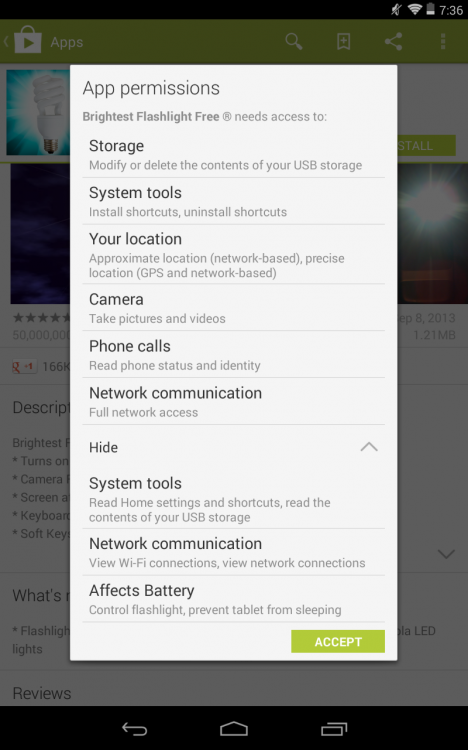
\includegraphics[width=0.8\textwidth]{img/brightestflashlight.png}
  \caption{The \emph{Brightest Flashlight Free} app prompting for it's permissions
    at install time.  This app is over privileged as a flashlight app should have
    no need for GPS or phone data, or network access.}
\end{marginfigure}

One criticism of the API permissions is that they are quite broad.  For instance
the \emph{internet} permission allows an app to send or receive anything on the
internet.  Several people have proposed a \emph{fine grained permissions model}
and developed tools to support it.  The \emph{RefineDroid, Dr.~Android \&
  Mr.~Hyde} tools\cite{Jeon:2012ki} are a suite designed to discover which
permissions can be made fine-grained, rewrite apps to use these permissions and
then enforce them at runtime; they do this on a stock Android system without
requiring rooting or kernel modification. Alternately the \emph{AppFence}
tool\cite{Hornyack:2011wq} works without modifying apps.  It allows users to
write fine grained policies for what data an app can receive: if an app exceeds
its bounds then the request is either denied or fake data supplied in its place.
This does require modifications to the Android OS however.  The \emph{AppGuard}
tool\cite{Backes:2013ec} offers something in between: it rewrites apps to use a
security monitor to enforce security policies at runtime.


\subsection{Intents and Collusion}

Android uses a novel IPC mechanism called \emph{Binder}.  Apps use
\emph{intents} to share data and handle events.  For instance if an app wishes
to handle an \code{SMS_RECEIVED} action it can declare itself a \emph{broadcast
  receiver} for it and the app will be started when the event occurs.
Alternatively if an app wants to open a URL in the browser it can send an
\code{ACTION_VIEW} intent and the user's chosen browser will take open the
URL.\@ Apps can create their own intents and can restrict usage of them (if they
wish) to only a limited number of other apps (or those signed with a specific
key).

These mechanisms also allow apps to collude to increase their privilege levels,
or share data inappropriately.  To do this consider the case where there are two
apps communicating: one which can use the network and another which cannot.  If
the unprivileged app asks the privileged app to send data on its behalf, and the
privileged app forwards the network responses back to it; then the unprivileged
app has the network permission without needing to declare it to the user.
Alternately if a privileged app does not secure its intents then they may break
the protections offered by permissions.  An example of this was the \emph{Kies}
app on Samsung~Galaxy~S3 phones that could be exploited to allow any app to
install other apps\cite{moulu:8btkPowj}.

Several tools have been developed to detect these privilege escalation attacks
such as \emph{Quire}\cite{Bugiel:2012ui} that added origin tracing to intents.
Other tools such as \emph{ScanDroid}\cite{Fuchs:2009vi} statically analyze apps
to find data-flows across components and produce a series of constraints that
should be satisfied to guarantee information security.  The
\emph{Kirin}\cite{Enck:2009ko} tool certifies apps at install time against a
policy based on the potential data-flows introduced by the permissions they
request.

The \emph{TaintDroid}\cite{Enck:2010uw} and \emph{FlowDroid}\cite{Fritz:2013vi}
have both had a large impact.  Both tools both use taint analysis to track the
data passed between apps and detect when sensitive data is being leaked to an
app that should not have access to it through intents, however others have shown
that the approach is not perfect\cite{Sarwar:2013ta} and can be defeated by
malicious apps.

% TODO: INCLUDE SECTION ON ANDROID ROMS AND MALWARE

\section{Policy Languages}

When an action is performed, such as reading a file or installing an app, there
are a set of conditions that must be met for the action to go ahead.  These
conditions form the \emph{authorization~policy} for that decision.  When these
policies describe what actions are permissible in order to maintain a secure
system then we call it the \emph{security~policy}.  

The policies often contain a notion of \emph{trust} where certain principals
may be trusted to make statements about other principals and what is
permissible.  To model the relationships many logics have been proposed that can
be implemented to decide whether an action can be authorized automatically.

Early authorization logics, such as \emph{PolicyMaker}\cite{Blaze:dj} grew out
of the logics of authentication proposed by
\citeauthor*{Wobber:1994dh}\cite{Lampson:1992jg}\cite{Wobber:1994dh}.
PolicyMaker allowed authorities to declare trust in other principles (identified
through asymmetric keys) for certain actions or to declare further trust
relationships.  The language was designed to be minimal and did not specify how
the policies should be checked: they suggested by using regular expressions, or
checking programs written in a sandboxed version of AWK however any language
could have been used. The author suggested that the language might be good as a
model for the public-key infrastructure.  Later work introduced
\emph{KeyNote}\cite{Blaze:1999fa} which they claimed was a simplified version of
PolicyMaker designed to support public-key infrastructure.

Later other languages such as \emph{RT}\cite{Li:2002if} were introduced.  RT
allowed principals to be given roles (in a manner similar to an \ac{RBAC}
access-control system) and for decisions to be made based on which roles an
entity held.  This meant that RT could express general statements that were not
expressible in the PolicyMaker languages such as:
\begin{quote}
  ``Anyone who is a preferred customer and a student can get a discount.''
\end{quote}
Several different versions of RT were described: the simplest being
\emph{RT$_0$}\cite{Li:2003tj} and with \emph{RT$_1$} and \emph{RT$_2$} adding support for
parameterized-roles and logical-objects respectively; each with extensions to
provide other features.

By providing a translation into \emph{Datalog} (specifically \emph{Datalog with
  constraints} or \emph{Datalog$^C$\cite{Li:2003ix}}), the RT family of
languages was shown to be tractable, unlike earlier languages.  Datalog is a
query language similar to \emph{Prolog} but that doesn't support nested
sub-queries or functions and has a safety condition\footnote{All variables in
  the head must occur in the body.}.  Datalog is a subset of first-order logic
and is known to be tractable: i{.}e{.} all queries can be done in polynomial
time.

Influences form the RT family of languages and Datalog$^C$ can be seen in the
\emph{Cassandra} policy rule language\cite{Becker:2004fi}.  Cassandra was a
trust management system that could be used to model large complicated systems.
In his doctoral thesis Becker showed how the NHS Spine (a complex and informally
defined system concerning access control and roles in health care) could be
formally modelled in the Cassandra language.  

In Cassandra principals activate and deactivate roles. Actions can only be completed if the
principal holds the required roles.  Delegation is allowed through an
appointment mechanism where one principal can activate a role on another
principal.  Like the RT languages Cassandra is tractable as it can be translated
to Datalog$^C$.

\begin{marginfigure}\label{code:cassandra}
  \begin{align*}
    &\textsf{canActivate}(mgr, \texttt{AppointEmployee}(emp)) \\ 
    &\;\;\gets \textsf{hasActivated}(mgr, \texttt{Manager}()) \\
    &\textsf{canActivate}(emp, \texttt{Employee}(app)) \\
    &\;\;\gets \textsf{hasActivated}(app, \texttt{AppointEmpolyee}(emp))
  \end{align*}
  \caption{Role delegation in the \emph{Cassandra} policy language. A manager is
  allowed to activate the employee role for an arbitrary entity by appointing
  them.}
\end{marginfigure}

The \emph{Binder} language\cite{DeTreville:2002ff} was designed for authorization
decisions\cite{Abadi:2003kt} and implemented as an extension of Datalog.
Properties are given to entities by creating arbitrary predicates for them, and
a special \emph{says} modality allows statements to be imported from third
parties.

\begin{marginfigure}\label{code:binder}
  \begin{lstlisting}[language=Prolog,morekeywords={*,says,:-},basicstyle=\scriptsize]
can(X, read, file) :- employee(X, company). 
employee(X, company) :- hr says empolyee(X, company).
hr says employee(john, company).
  \end{lstlisting}
  \caption{Statements in \emph{Binder} to say that in the current context only
    employees can read a file, and that an employee they must have a statement
    from HR to prove they are an employee.}
\end{marginfigure}

Authorisation is granted by checking to see if a predicate can be deduced from
the knowledge base, however because Binder does not add any special predicates,
and Datalog does not allow functions there can be no notion of state.

\subsection{{SecPAL}}

The \emph{{SecPAL}} authorization language\cite{Becker:2006vh} is an authorization
logic for decentralized systems.  Early experiments indicate that it is highly
suitable for modeling the distributed nature of software installation, app
stores and mobile devices so we will describe it in more detail than other
authorization languages.

Syntactically {SecPAL} appears similar to Binder, however it has a richer syntax
that allows for constraints and decisions to be made based on state (such as the
time).  {SecPAL} was designed to be readable and has a more verbose, English like,
language than other authorization logics. 

Like Binder it contains a \emph{says} statement however unlike Binder it
requires that all statements are said by a principal explicitly rather than
relying on a default context.  {SecPAL} also allows arbitrary predicates to be
created, and also adds two additional special modalities to the logic.  The
\emph{can-say} statement allows for explicit delegation and has two varieties.
The \emph{can-say$_\infty$} phrase allows for nested delegation, whereas the
\emph{can-say$_0$} statement does not.  {SecPAL} also adds a \emph{can-act-as}
phrase that allows for aliasing entities.

Later extensions of {SecPAL}\cite{Becker:2009vt} add support for guarded
universal quantification and remove the \emph{can-act-as} statement.  Other
languages such as \emph{DKAL}\cite{Gurevich:2008fz} built and eventually split
from {SecPAL}.  DKAL was designed to express distributed knowledge between
principals by adding to the trust delegation mechanisms already in {SecPAL}.
They also showed how any {SecPAL} statement could be translated into {DKAL}.
The \emph{{SecPAL}4P} language\cite{Becker:2009ula} was an instantiation of (the
extended version of) {SecPAL} designed to specify how users' wished their
\ac{PII} to be handled.

The inference rules for SecPAL are shown in Figure~\ref{secpal:rules}.  Queries
are evaluated against a set of known statements (the \ac{AC}) and an initially
infinite delegation level ($D$).  If the rules show that the query is valid then
SecPAL says the statement is okay else it is rejected.

\begin{figure}\label{secpal:rules}
  \begin{eqnarray*}
    \infer[\textsf{\scriptsize cond}]{%
      AC, D \models A\textsf{~says~}fact\theta
    }{%
      \begin{array}[c]{c}
        \left(A\textsf{~says~}\textit{fact}\textsf{~if~}\textit{fact}_1, \ldots, \textit{fact}_k, c\right) \in AC \\
        AC,D\models A\textsf{~says~}\textit{fact}_i\theta \; \forall i \in \{1\cdots k\} 
      \end{array}
      & \models{c\theta}
      & \textsf{vars}(\textit{fact}\theta) = \emptyset)
    }\\
    \infer[\textsf{\scriptsize can say}]{%
      AC, \infty \models A\textsf{~says~}\textit{fact}
    }{%
      AC, \infty \models A\textsf{~says~}B\textsf{~can~say}_D \textit{fact} 
      & AC, D \models B\textsf{~says~}\textit{fact}
    } \\
    \infer[\textsf{\scriptsize can act as}]{%
      AC, D \models A\textsf{~says~}B~\textit{verbphrase}
    }{%
      AC, D \models A\textsf{~says~}B\textsf{~can~act~as~}C
      & AC, D \models A\textsf{~says~}C~\textit{verbphrase}
    }
  \end{eqnarray*}
  \caption{The inference rules used to evaluate {SecPAL}. All {SecPAL} rules are
  evaluated in the context of a set of other assertions $AC$ as well as an
  allowed level of delegation $D$ which may be $0$ or $\infty$.}
\end{figure}


 
\end{document}

